\documentclass[First Project.tex]{subfiles}

\begin{document}


\section{ Άσκηση 2 }
Στην \textbf{2η άσκηση} ζητείται να υλοποιηθούν κάποιες παραλλαγές των μεθόδων της \textbf{1ης άσκησης} ενώ 
στην συνέχεια μας δίνεται η συνάρτηση 
\begin{equation*}
    f(x) = 94cos^{3}x - 24cosx + 177sin^{2}x - 108sin^{4}x -72cos^{3}xsin^{2}x - 65
\end{equation*}
και ζητείται να βρεθούν όλες οι ρίζες της στο διάστημα \textbf{[0,3]}. Αρχικά, σχηματίζουμε και πάλι την γραφική παράστασης της νέας
συνάρτησης :
\begin{figure}[h!]
    \centering
    \captionsetup{justification=centering}
    \begin{center}
        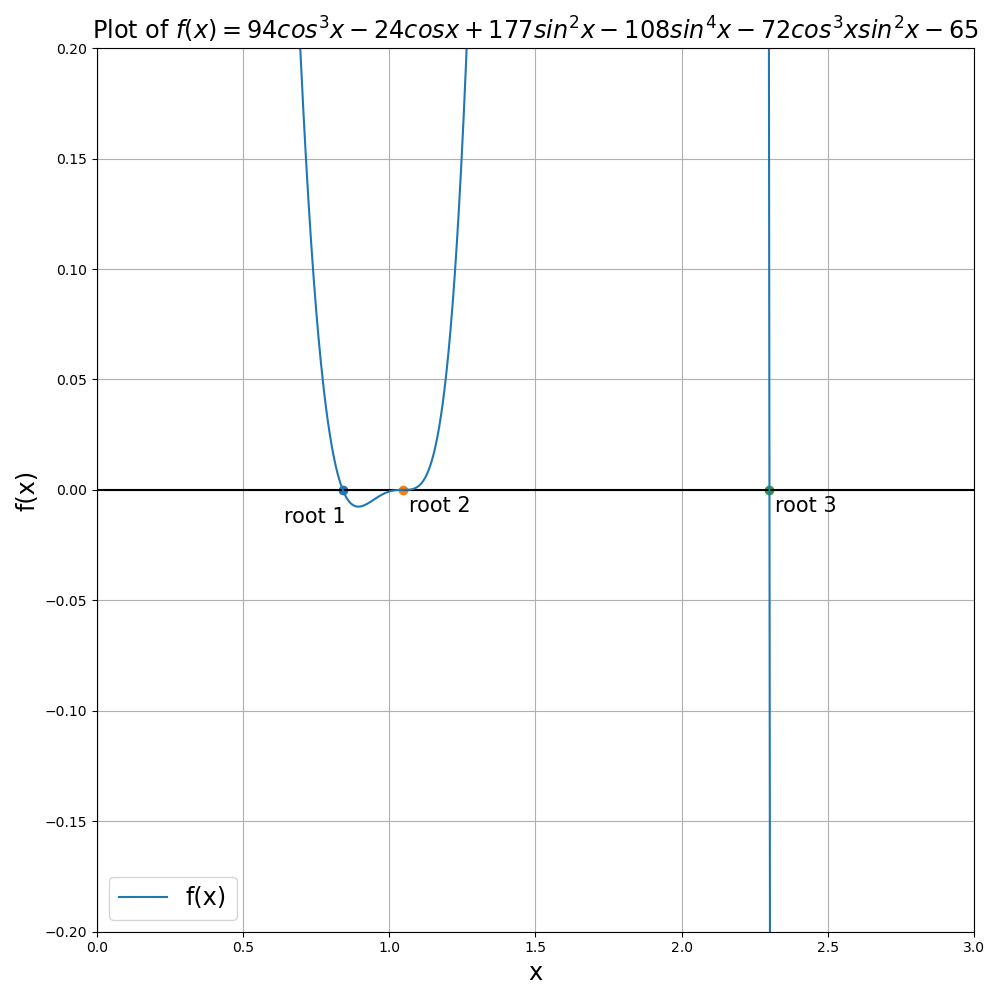
\includegraphics[scale=0.40]{exercise_2_function.png}    
        \caption{Γραφική παράσταση της συνάρτησης \textlatin{\textbf{f(x)}}}
    \end{center}
\end{figure}

Από την οποία παρατηρούμε στο \textit{Σχήμα 27} ότι η συνάρτηση έχει 3 ρίζες στο διάστημα \textbf{[0,3]}.


\end{document}